\documentclass[12pt]{article}
%\usepackage{Rd,Sweave,upquote}
\usepackage[reqno]{amsmath}
\usepackage{natbib,amssymb,amsthm,graphicx,verbatim,url,verbatim}
\usepackage[all]{xy}
\usepackage{vmargin}
\setpapersize{USletter}
\topmargin=0in
\usepackage{times}
\usepackage{dcolumn, booktabs}
\usepackage[dvipsnames,usenames]{color}
\usepackage{dcolumn}
\newcolumntype{.}{D{.}{.}{-1}}\newcolumntype{d}[1]{D{.}{.}{#1}}
%\usepackage[notref]{showkeys}
%\usepackage{endfloat}

\usepackage{color,setspace}
\definecolor{spot}{rgb}{0.6,0,0}
\usepackage[pdftex, bookmarksopen=true, bookmarksnumbered=true,
  pdfstartview=FitH, breaklinks=true, urlbordercolor={0 1 0},
  citebordercolor={0 0 1}, colorlinks=true, citecolor=spot, 
  linkcolor=spot, urlcolor=spot,
  pdfauthor={Gary King},
  pdftitle={}]{hyperref}

%squeeze
% == spacing between sections and subsections
%\usepackage[compact]{titlesec} 
% keep floats on same page
\renewcommand{\topfraction}{0.85}
\renewcommand{\textfraction}{0.1}
\renewcommand{\floatpagefraction}{0.75} % keep < \topfraction

\usepackage{soul}

\usepackage{appendix}
\usepackage{latexsym}
\newtheorem{claim}{Claim}
\newtheorem{proposition}{Proposition}
\newtheorem{theorem}{Theorem}
\newtheorem{lemma}{Lemma}
\newtheorem*{ass}{Assumption}
\newtheorem{question}{Question}
\newtheorem{remark}{Remark}
\newtheorem{definition}{Definition}
\newcommand{\bX}{\boldsymbol{X}}

\title{Estimates of Racial Differences in the Percent of Citizens to
  be Disenfranchised by the Texas Voter ID Law} \author{Gary
  King\thanks{Alfred J.  Weatherhead III University Professor, Harvard
    University, Institute for Quantitative Social Science, 1737
    Cambridge Street, Cambridge MA 02138; http://GKing.harvard.edu,
    king@harvard.edu, (617) 500-7570.}}

%\date{January 25, 2011}

\begin{document}
\maketitle
\tableofcontents
\clearpage
\doublespacing

\section{Introduction}

The purpose of this report is to estimate the differential percentages
of black, white, and Hispanic citizens of voting age who would be
disenfranchised (not allowed to vote) solely because they do not meet
the additional requirements of the new Texas Voter ID law.

The report from the Department of Justice’s expert Stephen
Ansolabehere examines the differential percentages of black, white,
and Hispanic \emph{registered voters} who would be disenfranchised by
the new law.  We supplement this information by attempting to estimate
the broader percentages disenfranchised of \emph{all} those in each
racial group who would have been eligible to vote without the new law,
including those who had and had not voted previously.  We also use
different assumptions and methods than Ansolabehere, the uncertainties
of which are likely uncorrelated with those from his report.  The
result is that the combination of the two reports should provide
stronger inferences than either alone.

\section{Background and Qualifications}

I am the Albert J Weatherhead III University Professor at Harvard
University, one of 24 with the designation of University Professor.  I
have taught at Harvard since 1987 and before that at New York
University.  I hold a Ph.D. from the University of Wisconsin.  I have
been elected a member of six honorary societies (National Academy of
Sciences 2010, American Statistical Association 2009, American
Association for the Advancement of Science 2004, American Academy of
Arts and Sciences 1998, Society for Political Methodology 2008, and
American Academy of Political and Social Science 2004), and have won
more than 30 ``best of'' awards for my articles, books, conference
papers, and software, among others.  I have published more than 130
journal articles, 15 open source software packages, and 8 books
spanning most aspects of political methodology, several fields of
political science, statistics, and other scholarly disciplines.  I
have served on more than 30 editorial boards.  The statistical methods
and software I developed are used extensively in litigation, academia,
government, consulting, and private industry.  More information on me
and copies of most of my work is available at
\url{http://gking.harvard.edu}.

I have been a expert witness or consultant (for governments and
partisans on both sides) in many U.S.\ states for legislative
redistricting and other matters.  Most recently, I was the expert for
the Arizona Independent Redistricting Commission.  I filed an Amici
Curiae brief in \emph{LULAC v. Perry} with three other scholars, which
was discussed and positively evaluated in three of the Supreme Court's
opinions, including the plurality decision.

\section{Methodological Approach}\label{s:methods}

In this section, we offer an overview of our methodological approach.
We will attempt to estimate the percentage of blacks, whites,
hispanics, and others who have valid voter identification, according
to the new Texas Voter ID law.  

From U.S.\ Census Data, we compute the percent of citizens' of voting
age who are black, white, hispanic, or other in each zip code area in
Texas.  Then from the State of Texas' driver's license database, we
compute the number of citizens of voting age (of any race) who have
valid identification, and from the combination of the two databases
the percent of citizens of voting age who have a valid ID.  

As there exists no data base to provide a complete cross-tabulation of
these results at the individual level, we use methods of ecological
inference --- which is the process of inferring from group level data
to information about individuals.  We summarize here the methods of
ecological inference we use.

In 1953, two methods of ecological inference were introduced --- the
method of bounds \citep{DunDav53} and ecological regression
\citep{Goodman53}. A special case of the method of bounds is known as
``homogeneous precinct analysis,'' which had been used in many court
cases: this approach seeks out ethnically homogeneous precincts (100\%
black or 100\% white, or 100\% Hispanic) because for those precincts
we know for certain the behavior of interest (in this case the percent
of those with a valid ID) of that one ethnic group.  The assumption
behind this method is that the percent with an ID observed in
homogeneous precincts is identical to that in other areas. The
advantage of this method is that it yields completely certain
information about some subgroups of citizens in some areas; the
disadvantage is that the relatively few who live in racially
homogeneous precincts may have starkly different proportions of IDs
than the vast majority of the population who live in (at least
partially) heterogeneous areas.  The method of bounds is more general
than homogeneous precinct analysis because the former can also provide
some information about heterogeneous precincts; it does this in the
form of ``bounds'' or ranges into which the fraction of a minority
group having IDs must fall.

The second method of ecological inference --- ecological regression
--- ignores the information revealed by the method of bounds and its
special case of homogeneous precinct analysis. Instead, ecological
regression uses statistical information across all precincts. For
example, if we find in areas with more African Americans that fewer
people have voter IDs, then we may be willing to infer that it is the
African Americans who have fewer IDs. The advantage of this approach
is that it uses some information from all precincts. The disadvantage
is that the information can be misleading: For example, also
consistent with the same evidence would be that the (perhaps poor)
whites who live in areas with high African Americans concentrations
are the ones with fewer IDs. In fact, as an indication of the common
problems with this method, ecological regression, unlike the method of
bounds, regularly gives impossible answers -- such as estimating the
percent of Hispanics voting for the Democrats as 120\% or $-54$\%.

The method of bounds (or homogeneous precinct analysis) and ecological
regression dominated the academic literature and courtroom expert
testimony from 1953 until 1997 when the approach known as EI was
introduced \citep{King97}. This approach was the first to combine the
deterministic information from the method of bounds with the
statistical information from ecological regression into a single set
of estimates. Thus, it uses the statistical information from all
precincts, the certain information from homogeneous precincts, and
other deterministic information known for certain from other precincts
(given in the form of ranges of estimates).  Impossible estimates are
never produced by this methodology, and all information from all
precincts are used in the analysis. Like any indirect method of
revealing information about individuals from aggregate data, EI is
also uncertain to a degree, but it uses more information than other
previous approaches.

Since EI was introduced, a variety of other methods have been
developed in the academic literature, virtually all of which follow
the same practice of including deterministic and statistical
information in the same model.  For example, \citet{RosJiaKin01}
extend King's method to large numbers of ethnic groups and candidates;
we use this method in our work as well as King's original method. Some
of the other methods of ecological inference have been collected in the
edited volume by \citet{KinRosTan04b}.

In practice, when we have data we can use to validate the methods,
ecological regression and homogeneous precinct analysis are often
inaccurate in many situations. Studies have shown that uncertainty
remains with King's and other subsequent methods --- which will always
be the case because some information is lost in the process of
aggregate --- but the estimates are usually superior. Differences
among the new methods that include both deterministic and statistical
information are, in comparison, relatively minor.

In this case, we use these newer methods to give estimates of the
proportion of each ethnic group that has a valid voter ID.  We also
use King's ``tomography plots'' and other diagnostic methods that help
us discern when adjustments in the methods need to be made, and how
much uncertainty remains.

The ecological inference methods we use here have the advantage of
avoiding any error that may otherwise be introduced in matching voter
registration files with the driver's license database and using the
Catalyst data to ascertain the race of voters who do not have IDs (and
so are not in the State Driver's license data base).  In addition, we
are able to estimate the percent of all citizens of voting age who
have IDs, rather than only those who are presently registered.
Although one cannot vote without being registered, in future elections
those not registered now of course do have the choice of registering.

\subsection{An Explication of Sample Ecological Inference Results}

We used our approach to ecological inference to determine the extent
of racially polarized voting in Arizona as well as the electability of
each district's candidate of choice among minority voters. For each
congressional district in the existing (i.e., ``benchmark'') and
proposed map, we estimated the turnout for each minority group and the
proportion of each minority group's vote for each candidate. 

To illustrate our approach, we describe the analysis for the vote
totals for a single election occurring in a single congressional
district.  Thus, Table~\ref{smine_cvap_cd_3_ex} displays estimates of
how each racial group in the proposed Congressional District 3 voted
in the 2010 election for Arizona Mine Inspector. Note that in each
table the total population in the last column and the total votes in
the last row are {\it observed} while the internal cells are {\it estimated} 
by our methodology. The bottom row labeled Total Pop
gives the population vote totals computed by aggregating over all VTDs
in the district.  Similarly, the column labeled Total CVAP lists the
share of citizen voting age population comprised by each racial group
in the district.  Again, this is calculated by simply aggregating over
all VTDs in the district.

\begin{table}[ht]
\begin{center}
\caption{\label{smine_cvap_cd_3_ex}Mine Inspector 2010 CD 3 (Proposed)}
\begin{tabular}{lccccc}
  \hline
Racial Group & Turnout & D Vote & R Vote & S Vote & Total CVAP\\ 
  \hline
White & 0.36 & 0.35 & 0.65 & 0.00 & 0.43 \\ 
  Hispanic & 0.30 & 0.90 & 0.10 & 0.00 & 0.44 \\ 
  Native American & 0.22 & 0.90 & 0.09 & 0.01 & 0.04 \\ 
  Black & 0.13 & 0.50 & 0.48 & 0.02 & 0.05 \\ 
  Other & 0.21 & 0.55 & 0.44 & 0.01 & 0.05 \\ 
  Total Pop & 0.31 & 0.61 & 0.39 & 0.00 &  \\ 
   \hline
\end{tabular}
\end{center}
\end{table}

The internal cells in the table contain estimates from ecological
inference. For example, we estimate that 90\% (0.90 in the table) of
Hispanic citizens in CD 3 voted for the Democratic Candidate and 10\%
for the Republican candidate (and 0\% for any third party candidates).
Furthermore, we know that Hispanics made up 44\% of the district's
total population (CVAP) and we estimate that they turned out for the
election at a rate of 30\%.  Looking at the district as a whole, we
observe that the Democratic candidate received 61\% of the vote. 

%Thus, on the basis of the quantitative information from the 2010 Mine Inspector election in the proposed CD 3, the Democratic candidate
%seems to be the candidate of choice for Hispanic voters and this
%candidate comfortably carried the district despite the existence of
%some level of polarized voting --- that is, lower support among white
%voters who we estimate voted for the Democrat at a rate of only 35\%
%compared to the Hispanics 90\%.

%As an illustration of our method of analysis, we now describe how we determine the level of racially polarized voting as well as the ability to elect the candidate of choice for this district.

To judge the level of racial polarization in CD 3, we examine the
differences in the voting patterns of whites and Hispanics. In this
district, we estimate that the Democratic candidate received 35\% of
the vote among white voters; on the other hand, the Democrat received
90\% of the vote among Hispanic voters. Because of this wide
discrepancy, along with the fact that the majority of white voters
preferred a different candidate than the majority of Hispanic voters,
we conclude that racially polarized voting exists in CD 3 for this
election.

We now describe how we judge the level of support among the main
minority for the candidate of choice, as well as whether the district
as a whole is strong enough to elect this candidate. In CD 3 the
expected candidate of choice is the Democratic candidate, who is also
Hispanic. The data appear to confirm this hypothesis, as 90\% of
Hispanic voters preferred the Democratic candidate. After confirming
the level of support for the candidate of choice, we turn to the
district wide support for this candidate. In this case, 61\% of all
voters in proposed CD 3 voted for the candidate of choice. This level
of support provides a comfortable margin of victory. Therefore, we
conclude that Hispanics in proposed CD 3 have a clear candidate of
choice and furthermore that the district as a whole demonstrates the
ability to elect this candidate.

This example illustrates the method of analysis for a single race in a
single district. We conducted this form of analysis for each district
in each election of interest. In the sections that follow, we use our
estimates for each district and election to assess the level of racial
polarization and ability to elect the candidate of choice.  The
results presented here use the Citizen Voting Age Population (CVAP)
totals. We present the same set of estimates using Voting Age
Population (VAP) totals in the digital appendix.  We have included
tables illustrating the estimates for each district and each race in
the appendix of this report.

\subsection{Sources of Uncertainty}

There are several sources of uncertainty in ecological inference
estimates including estimation uncertainty, fundamental uncertainty,
and model dependence.  \emph{Estimation uncertainty} occurs because we
have a limited set of observations (zip code areas) to use in
estimating the disenfranchisement rates for each racial group votes.
\emph{Fundamental uncertainty} is the idea that even with a large
amount of data there is some degree of randomness in the process of
signing up to get a driver's license or ID.  A citizen's license
expires inadvertently, or they forget to sign up, or their name is
typed into the database incorrectly, or racial group information is
mis-estimated by the Census bureau; this is the stuff of measurement
and human behavior and is modeled in a well-known way as fundamental
variability.  Finally, \emph{model dependence} is the degree to which
changes in modeling assumptions affect our estimates.  Models are
required in ecological inference because some information is destroyed
in the process of aggregation and kept from the analyst without having
full information on every individual in the state.

In different types of statistical problems, each of these sources of
uncertainty can play difference roles and to differing degrees.
Ecological inferences of course have all three sources of uncertainty,
but it is the model dependence caused by having to estimate voter ID
rates because all information is not in the public domain that
accounts for the overwhelming fraction of overall uncertainty.  Model
dependence typically dwarfs the other two components. Thus, we tune
our methods of assessing uncertainty to focusing on model dependence.

To convey the degree of uncertainty in the estimates of turnout and
vote share, we use ``tomography plots'' to accompany the tables.
These plots give all information in the data without making any
statistical modeling assumptions, as well as summarizing the available
statistical information in the data. This enables us to evaluate
directly how much information is available in the data and how much
is imposed by the statistical model.

One entire tomography plot is needed for each numerical estimate in
the corresponding table. For one example, the tomography plot in
Figure \ref{tomog} analyzes the information and uncertainty in the
data and our analyses with respect to two unknowns: the percent of
Whites (horizontally) and non-Whites (vertically) who vote for the
Hispanic candidate in District 3, in each precinct.  If these two
quantities were known for a precinct, they would appear in the plot as
a single dot, and the set of precincts as a set of dots.  However,
because of the secret ballot, we cannot know any of the exact points
with precision; what the plot shows is that the information hidden
from us by the secret ballot is directly quantifiable: it turns each
precinct's dot into a line.  We can think of the dot as being smeared
into a line. That smearing represents a loss of information, but much
information is retained (and that is uniquely captured by our methods
of ecological inference).  In particular, we know for certain that the
true point representing the percent of whites and non-whites who vote
for the Hispanic candidate falls somewhere on the line; we do not know
where on the basis of just the information from that precinct, but we
know it must be on the line.

\begin{figure}[htb]
\begin{centering}
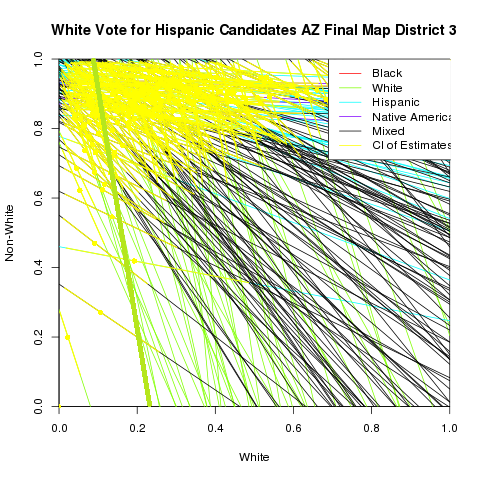
\includegraphics[scale=1]{figs/pl_whitevote_h_3.png}
\caption{\label{tomog}This tomography plot displays the white vote
  for the Hispanic Candidate in 2010 Mine Inspector Election
  (horizontally) by non-white vote for the same election (vertically)}
\end{centering}
\end{figure}

For example, consider the bold green line in the plot. We know, based
on the observed data from that precinct (the percent voting and the
percent Hispanic), that the point in this plot (representing where the
White and non-White vote share is) for this precinct must be some
point on the line, but we do not know exactly where on the line this
point falls. For this line, we know that the fraction of Whites that
vote for the Hispanic candidate must fall somewhere between 0.16 (16
percent) and 0.23 (23 percent). We get these numbers by projecting the
line downwards to the horizontal axis. If instead we project the line
to the left (vertical) axis, we can see that, for this particular
precinct, the range of possible values for the percent of non-Whites
voting for the Hispanic candidate could be anywhere from 0\% to 100\%.
That estimate is better than the method of ecological regression,
which often gives answers outside that interval, but still we can see
that this precinct is informative with respect only to Whites, not
non-Whites. 

In this way, each line on a tomography plot captures exactly what we
do and do not know about the voting behavior in each precinct ---
without any uncertainty (assuming only that the data are measured
correctly). Our statistical method then uses all this available
information as well as the statistical information from ecological
regression. Lines that are relatively steep in this particular
tomography plot convey a lot of information about the percent of
Whites that vote for the Hispanic candidate.  Lines that are
relatively flat convey a great deal of information about the percent
of non-Whites voting for the Hispanic candidate.  Lines that cut off
the top right or bottom left corner of the plot are informative about
both quantities.

The tomography plots reflect what we know about the racial composition
of each precinct. If a precinct contains more than 65\% of a
particular racial group (which we use as an arbitrary cutoff for
graphical clarity), then the line on the tomography plot that
corresponds to that precinct is color coded to represent the majority
group (see the legend in the plot). If no groups comprise 65\% or more
of the precinct, then no color code is assigned.  

Finally, the tomography plots also reflect the results of the
ecological inference statistical estimation, that includes information
on patterns across precincts. The point estimate (i.e., the exact
point on the line that we estimate as the vote share for each group)
as well as the confidence intervals are colored yellow.  Taken
together, these describe the overall estimate of how racial groups
voted in the district as a whole. For example, in the tomography plot
for District 3 in Figure \ref{tomog}, the mass of yellow in the top
left means that our estimates indicate that whites voted for the
Hispanic candidate at a substantially lower rate than did their
non-white counterparts in the district.  

As importantly, the tomography plots convey the \emph{overall
  uncertainty} in the available data, and how our statistical
estimator uses that information to produce an estimate.  In this
particular example, the prevalence of flat lines near the top and
steep lines near the left convey a great deal of information about
where and what we are uncertain about.  The statistical estimator
assumes that there is some relationship among all the precincts in a
district, and so in all likelihood there exists a cluster of points on
the plot somewhere such that when two lines cross or approach one
another, the true points on each are close to each other on their
respective lines.  

To appropriately and completely judge all sources of uncertainty in
ecological inferences requires examining a plot like this for each
numerical quantity to be estimated.  The uncertainty estimates here
are far more informative and information rich than sampling based
confidence intervals or standard errors, which assume the model is
true and only summarize fundamental and estimation uncertainty.  Our
appendix includes all such plots, calculated for all offices we
analyzed, for VAP and CVAP, and for each district.



\section{Data}\label{s:data}

\section{Results}\label{s:res}

\singlespace
\bibliographystyle{apsr} 
\bibsep=0in 
%\phantomsection
\addcontentsline{toc}{section}{References}
\bibliography{gk,gkpubs}
\end{document}
